\section{互联网}

\subsection{什么是互联网}

计算机网络（简称为网络）由若干结点（node）和连接这些结点的链路（link）组成。网络中的结点可以是计算机、集线器、交换机或路由器等。网络之间还可以通过路由器互连起来，这就构成了一个覆盖范围更大的计算机网络。这样的网络称为互连网（internetwork或internet）。因此互连网是“网络的网络”（network of networks）。

\begin{figure}[htpb]
    \centering
    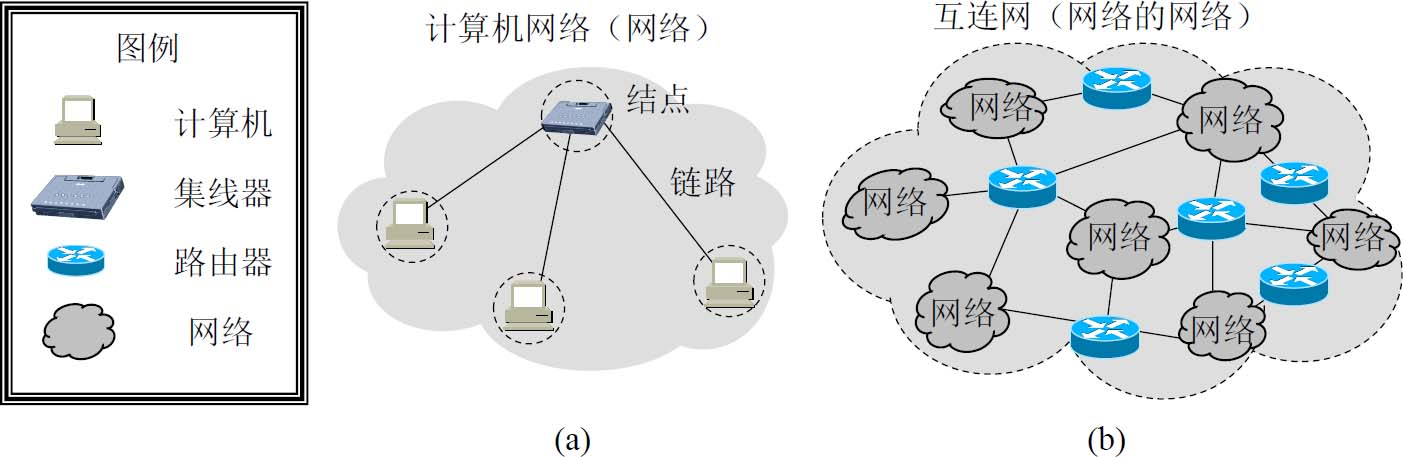
\includegraphics[width=\linewidth]{figures/Image00003.jpg}
\end{figure}

网络把许多计算机连接在一起，而互连网则把许多网络通过路由器连接在一起。与网络相连的计算机常称为主机。还有一点也必须注意，就是网络互连并不是把计算机仅仅简单地在物理上连接起来，因为这样做并不能达到计算机之间能够相互交换信息的目的。我们还必须在计算机上安装许多使计算机能够交换信息的软件才行。

\subsection{互联网基础结构发展的三个阶段}
\begin{enumerate}
    \item 从单个网络ARPANET向互连网发展
    
    1969年美国国防部创建的第一个分组交换网ARPANET最初只是一个单个的分组交换网（并不是一个互连的网络）。所有要连接在ARPANET上的主机都直接与就近的结点交换机相连。但到了20世纪70年代中期，人们已认识到不可能仅使用一个单独的网络来满足所有的通信问题。于是ARPA开始研究多种网络（如分组无线电网络）互连的技术，这就导致了互连网络的出现。这就成为现今互联网（Internet）的雏形。1983年TCP/IP协议成为ARPANET上的标准协议，使得所有使用TCP/IP协议的计算机都能利用互连网相互通信，因而人们就把1983年作为互联网的诞生时间。1990年ARPANET正式宣布关闭，因为它的实验任务已经完成。
    \item 三级结构的互联网
    
    从1985年起，美国国家科学基金会NSF（NationalScienceFoundation）就围绕六个大型计算机中心建设计算机网络，即国家科学基金网NSFNET。它是一个三级计算机网络，分为主干网、地区网和校园网（或企业网）。这种三级计算机网络覆盖了全美国主要的大学和研究所，并且成为互联网中的主要组成部分。1991年，NSF和美国的其他政府机构开始认识到，互联网必将扩大其使用范围，不应仅限于大学和研究机构。世界上的许多公司纷纷接入到互联网，网络上的通信量急剧增大，使互联网的容量已满足不了需要。于是美国政府决定将互联网的主干网转交给私人公司来经营，并开始对接入互联网的单位收费。
    \item 多层次ISP结构的互联网
    
    从1993年开始，由美国政府资助的NSFNET逐渐被若干个商用的互联网主干网替代，而政府机构不再负责互联网的运营。这样就出现了一个新的名词：互联网服务提供者ISP（InternetServiceProvider）。在许多情况下，ISP就是一个进行商业活动的公司，因此ISP又常译为互联网服务提供商。例如，中国电信、中国联通和中国移动等公司都是我国最有名的ISP。

    ISP可以从互联网管理机构申请到很多IP地址（互联网上的主机都必须有IP地址才能上网，这一概念我们将在第4章的4.2.2节详细讨论），同时拥有通信线路（大ISP自己建造通信线路，小ISP则向电信公司租用通信线路）以及路由器等连网设备，因此任何机构和个人只要向某个ISP交纳规定的费用，就可从该ISP获取所需IP地址的使用权，并可通过该ISP接入到互联网。IP地址的管理机构不会把一个单个的IP地址分配给单个用户（不“零售”IP地址），而是把一批IP地址有偿租赁给经审查合格的ISP（只“批发”IP地址）。由此可见，现在的互联网已不是某个单个组织所拥有而是全世界无数大大小小的ISP所共同拥有的，这就是互联网也称为“网络的网络”的原因。
\end{enumerate}

\subsection{互联网+}
现在常常可以看到一种新的提法，即“互联网+”。它的意思就是“互联网+各个传统行业”，因此可以利用信息通信技术和互联网平台来创造新的发展生态。实际上“互联网+”代表一种新的经济形态，其特点就是把互联网的创新成果深度融合于经济社会各领域之中，这就大大地提升了实体经济的创新力和生产力。我们也必须看到互联网的各种应用对各行各业的巨大冲击。例如，电子邮件迫使传统的电报业务退出市场。网络电话的普及使得传统的长途电话（尤其是国际长途电话）的通信量急剧下降。对日用商品快捷方便的网购造成了不少实体商店的停业。原来必须排长队购买火车票的网点已被非常方便的网购所替代。网约车的问世对出租车行业产生了的巨大冲击。这些例子说明了互联网应用已对整个社会的各领域产生了很大的影响。

中国国际“互联网+”大学生创新创业大赛是由教育部与政府、各高校共同主办的赛事。大赛要求参赛项目能够将移动互联网、云计算、大数据、人工智能、物联网、下一代通讯技术、区块链等新一代信息技术与经济社会各领域紧密结合，服务新型基础设施建设，培育新产品、新服务、新业态、新模式；发挥互联网在促进产业升级以及信息化和工业化深度融合中的作用，促进制造业、农业、能源、环保等产业转型升级；发挥互联网在社会服务中的作用，创新网络化服务模式，促进互联网与教育、医疗、交通、金融、消费生活等深度融合。

要从实际问题中来，到实际问题中去，来解决实际问题，项目创新点是一个项目的核心，能达到的最终高度关键取决于核心思路。

\section{网址是什么？}


{\bfseries \cgreen{网址（URL）的构成}}

URL : Uniform Resource Locator，统一资源定位符

https://www.hebau.edu.cn/info/1062/15713.htm

\begin{itemize}
    \item 协议：http
    \item 服务：www (万维网)
    \item 域名：hebau.edu.cn
    \item 网站类型：edu.cn
    \item 目录：info/1062
    \item 文件：15713.htm
\end{itemize}

{\bfseries \cgreen{常见网址协议(scheme)}}

\begin{itemize}
    \item http
    
    超文本传输协议（HyperText Transfer Protocol）

    互联网应用最广泛的一种网络协议，客户端和服务器端请求和答应的标准。
    \item https
    
    由于HTTP天生“明文”的特点，整个传输过程完全透明，任何人都能够在链路中截获、修改或者伪造请求/响应报文，数据不具有可信性。因此就诞生了为安全而生的HTTPS协议。这是加强版http协议，是一种更加安全的数据传输协议。
    \item ftp
    
    访问远程FTP服务器上的文件。
    \item file
    
    访问本地磁盘上的文件。
    \item mailto
    
    邮件地址协议
    
    HTTP 和 HTTPS 的协议名称后面，紧跟着一个冒号和两个斜杠（://）。其他协议不一定如此，邮件地址协议mailto:的协议名后面只有一个冒号，比如 mailto:foo@example.com。
\end{itemize}

{\bfseries \cgreen{端口}}

端口紧跟在域名后面，两者之间使用冒号分隔。

比如www.example.com:80。

\begin{table}[ht]
    \caption{默认端口}
    \centering
    \label{tab:my-table}
    \begin{tabular}{|l|l|}
        \hline
        http & 80 \\ \hline
    https & 443 \\ \hline
    ftp & 21 \\ \hline
    socks & 1080 \\ \hline
    \end{tabular}
    \end{table}

{\bfseries \cgreen{网站类型}}

.com 国际最广泛流行的通用域名格式

.cn 中国国家域名

.org 非赢利性组织

.edu 教育机构

.gov 国家政府机构


{\bfseries \cgreen{路径}}

路径（path）是资源在网站的位置。比如，/info/1062/15713.htm这个路径，指向网站的/info/1062子目录下面的网页文件15713.htm。

互联网的早期，路径是真实存在的物理位置。现在由于服务器可以模拟这些位置，所以路径只是虚拟位置。

路径可能只包含目录，不包含文件名，比如/foo/，甚至结尾的斜杠都可以省略。这时，服务器通常会默认跳转到该目录里面的index.html文件（即等同于请求/foo/index.html），但也可能有其他的处理（比如列出目录里面的所有文件），这取决于服务器的设置。一般来说，访问www.example.com这个网址，很可能返回的是网页文件 www.example.com/index.html。

\section{IP地址}

{\bfseries \cgreen{IP地址的格式}}

IP地址=网络地址+主机地址

\begin{figure}[ht]
    \centering
    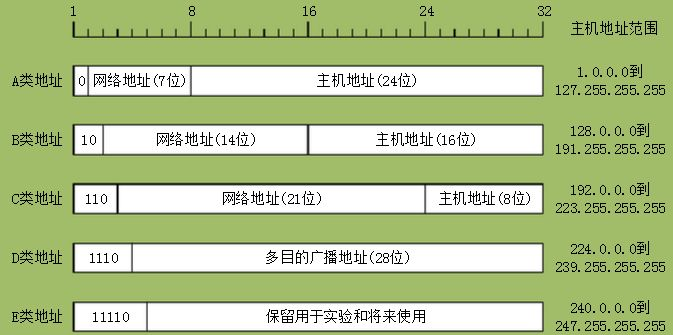
\includegraphics[width=\linewidth]{figures/IP.jpg}
\end{figure}

最初设计互联网络时，为了便于寻址以及层次化构造网络，每个IP地址包括两个标识码（ID），即网络ID和主机ID。同一个物理网络上的所有主机都使用同一个网络ID，网络上的一个主机（包括网络上工作站，服务器和路由器等）有一个主机ID与其对应。IP地址根据网络ID的不同分为5种类型，A类地址、B类地址、C类地址、D类地址和E类地址。

{\bfseries \cgreen{IP地址的分类}}

\begin{enumerate}
    \item A类IP地址
    
    个A类IP地址由1字节的网络地址和3字节主机地址组成，网络地址的最高位必须是“0”， 地址范围从0.0.0.0～126.255.255.255，默认子网掩码为：255.0.0.0。可用的A类网络有126个，每个网络能容纳1677多万个主机。A类地址分配给规模特别大的网络使用，例如IBM公司的网络。A类IP地址占IP地址总数比例1/2。
    \item B类IP地址
    
    一个B类IP地址由2个字节的网络地址和2个字节的主机地址组成，网络地址的最高位必须是“10”，地址范围从128.0.0.0到191.255.255.255，默认子网掩码为：255.255.0.0。可用的B类网络有16382个，每个网络能容纳6万多个主机 。B类IP地址占IP地址总数比例1/4。B类地址分配给一般的中型网络。
    \item C类IP地址
    
    一个C类IP地址由3字节的网络地址和1字节的主机地址组成，网络地址的最高位必须是“110”。范围从192.0.0.0到223.255.255.255，默认子网掩码为：255.255.255.0。C类网络可达209万余个，每个网络能容纳254个主机。 C类IP地址占IP地址总数比例1/8。C类地址分配给小型网络，如一般的局域网和校园网，它可连接的主机数量是最少的，采用把所属的用户分为若干的网段进行管理。
    \item D类IP地址
    
    用于多点广播（Multicast）。 D类IP地址第一个字节以“1110”开始，它是一个专门保留的地址。
    \item E类IP地址
    
    以“11110”开始，为将来使用保留。
\end{enumerate}

{\bfseries \cgreen{IP私有地址}}

私有IP就是在本地局域网上的IP，与之对应的是公有IP（在互联网上的IP）。

随着私有IP网络的发展，为节省可分配的注册IP地址，有一组IP地址被拿出来专门用于私有IP网络，称为私有IP地址。

在IP地址3种主要类型里，各保留了3个区域作为私有地址，其地址范围如下： 

A类地址：10.0.0.0～10.255.255.255 

B类地址：172.16.0.0～172.31.255.255 

C类地址：192.168.0.0～192.168.255.255

{\bfseries \cgreen{判断两个IP地址是否是同一个网段中}}

要判断两个IP地址是不是在同一个网段，就将它们的IP地址分别与子网掩码做与运算，得到的结果一网络号，如果网络号相同，就在同一子网，否则，不在同一子网。

例：假定选择了子网掩码255.255.254.0，现在分别将上述两个IP地址分别与掩码做与运算：

\begin{framed}
    211.95.165.24 11010011 01011111 10100101 00011000

    255.255.254.0 11111111 11111111 111111110 00000000

    与的结果是: 11010011 01011111 10100100 00000000

    211.95.164.78 11010011 01011111 10100100 01001110

    255.255.254.0 11111111 11111111 111111110 00000000

    与的结果是: 11010011 01011111 10100100 00000000
\end{framed}

可以看出,得到的结果(这个结果就是网络地址)都是一样的，因此可以判断这两个IP地址在同一个子网。

{\bfseries \cgreen{子网掩码}}

子网掩码是一个32位的2进制数， 其对应网络地址的所有位都置为1，对应于主机地址的所有位置都为0。子网掩码告知路由器，地址的哪一部分是网络地址，哪一部分是主机地址，使路由器正确判断任意IP地址是否是本网段的，从而正确地进行路由。

网掩码不能单独存在，它必须结合IP地址一起使用。子网掩码的主要作用有两个，一是用于屏蔽IP地址的一部分以区别网络标识和主机标识，并说明该IP地址是在局域网上，还是在远程网上。二是用于将一个大的IP网络划分为若干小的子网络。

\section{DNS域名系统}

{\bfseries \cgreen{一个疑问}}

首先我们要清楚以下几点：
\begin{itemize}
    \item 互联网上的所有数据都是存储在主机(服务器)上
    \item 互联网中的所有主机都拥有唯一的IP地址
    \item 互联网中任意两台主机通信都是通过IP地址来实现
\end{itemize}
\begin{framed}
    如何查看网站ip地址：

    cmd

    ping www.baidu.com
\end{framed}

我们以两台主机最简单的通信方式——上网为例，我们上网的实质就是获取网址对应主机上的数据并在用户主机上进行展示(浏览器上)，那么我们就该怀疑一个问题：互联网中的任意两台主机通信是依靠IP地址进行的，而我们上网只是输入的网址，并不是IP地址，怎么就能找到对方主机并获取它的数据呢?

{\bfseries \cgreen{域名系统}}

域名系统(Domain Name System, DNS)是因特网使用的命名系统，用来把便于人们记忆的具有特定含义的主机名(如www.example.com)转换为便于机器处理的IP地址。

相对于IP地址，人们更喜欢使用具有特定含义的字符串来标识因特网上的计算机。

\begin{figure}[ht]
    \centering
    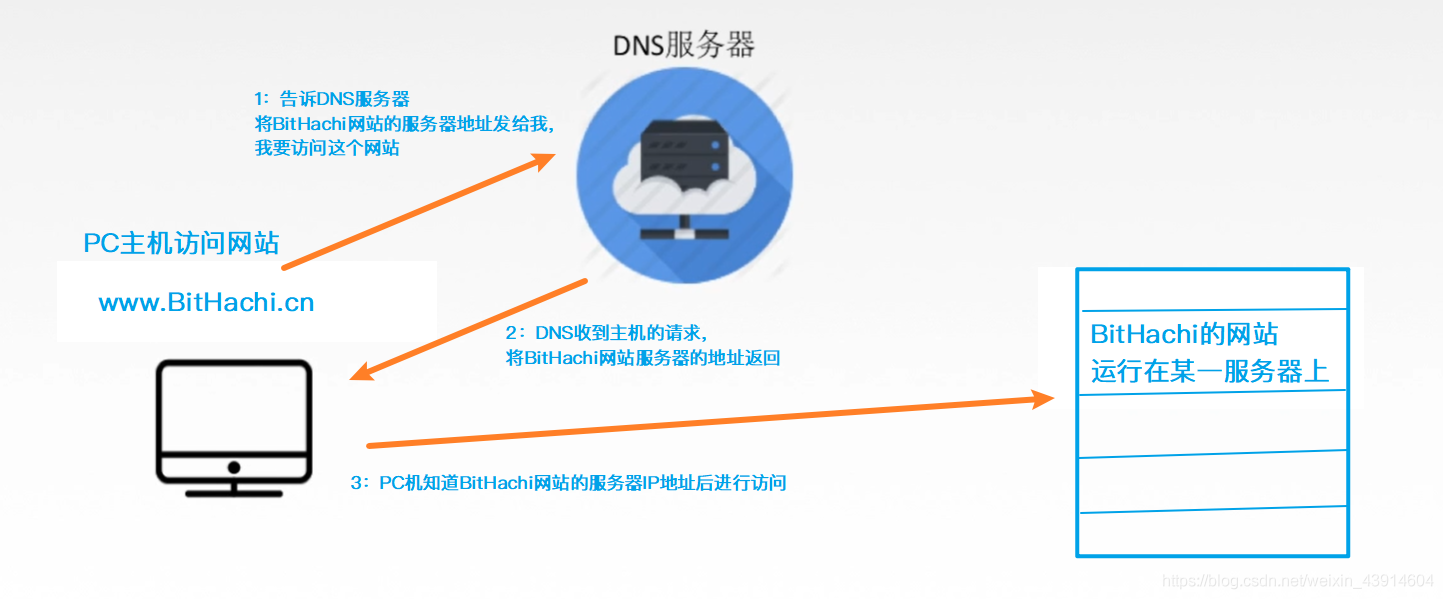
\includegraphics[width=\linewidth]{figures/dns.png}
\end{figure}

因特网采用层次树状结构的命名方法。采用这种命名方法，任何一个连接到因特网的主机或路由器，都有一个唯一的层次结构名称，即域名(Domain Name)。

域还可以划分为子域，而子域还可以继续划分为子域的子域，这样就形成了顶级域、二级域、三级域等。

{\bfseries \cgreen{域名服务器}}

因特网的域名系统被设计成一个联机分布式的数据库系统，并采用客户/服务器模型。

域名到IP地址的解析是由运行在域名服务器上的程序完成的。

每个域名服务器不但能够进行一些域名到IP地址的解析，而且还必须具有连向其他域名服务器的信息。当自己不能进行域名到IP地址的转换时，能够知道到什么地方去找其他域名服务器。

DNS使用了大量的域名服务器，它们以层次方式组织。没有一台域名服务器具有因特网上所有主机的映射，相反，该映射分布在所有的DNS上。

采用分布式设计的DNS，是一个在因特网上实现分布式数据库的精彩范例。主要有4种类型的域名服务器。

\begin{figure}[ht]
    \centering
    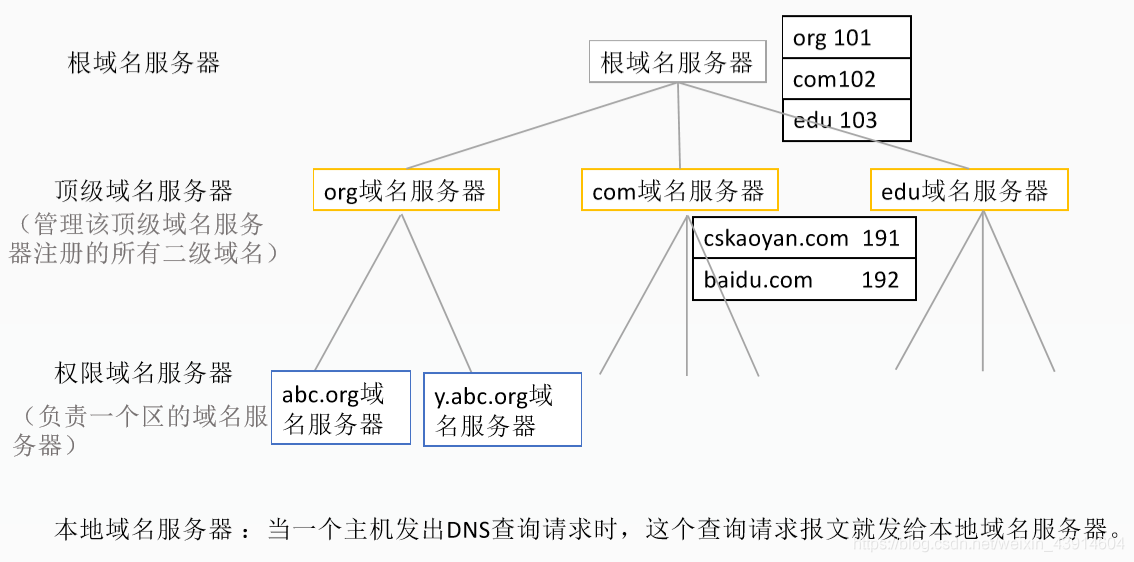
\includegraphics[width=\linewidth]{figures/dns-server.png}
\end{figure}

\begin{itemize}
    \item 根域名服务器
    
    根域名服务器是最高层次的域名服务器，所有的根域名服务器都知道所有的顶级域名服务器的IP地址。

    根域名服务器也是最重要的域名服务器，不管是哪个本地域名服务器，若要对因特网上任何一个域名进行解析，只要自己无法解析，就首先要求助于根域名服务器。

    根域名服务器用来管辖顶级域(如.com)， 通常它并不直接把待查询的域名直接转换成IP地址，而是告诉本地域名服务器下一步应当找哪个顶级域名服务器进行查询。
    \item 顶级域名服务器
    
    这些域名服务器负责管理在该顶级域名服务器注册的所有二级域名。

    收到DNS查询请求时,就给出相应的回答
    \item 权限域名服务器
    
    每台主机都必须在授权域名服务器处登记。为了更加可靠地工作，一台主机最好至少有两个授权域名服务器。

    实际上，许多域名服务器都同时充当本地域名服务器和授权域名服务器。

    授权域名服务器总能将其管辖的主机名转换为该主机的IP地址。
    \item 本地域名服务器
    
    本地域名服务器对域名系统非常重要。

    每个因特网服务提供者(ISP)， 或一所大学，甚至一所大学中的各个系，都可以拥有一个本地域名服务器。

    当一台主机发出DNS查询请求时，这个查询请求报文就发送给该主机的本地域名服务器。

    事实上，我们在Windows系统中配置“本地连接”时，就需要填写DNS地址，这个地址就是本地DNS (域名服务器)的地址。
\end{itemize}

\cred{递归查询，迭代查询}

\begin{figure}[ht]
    \centering
    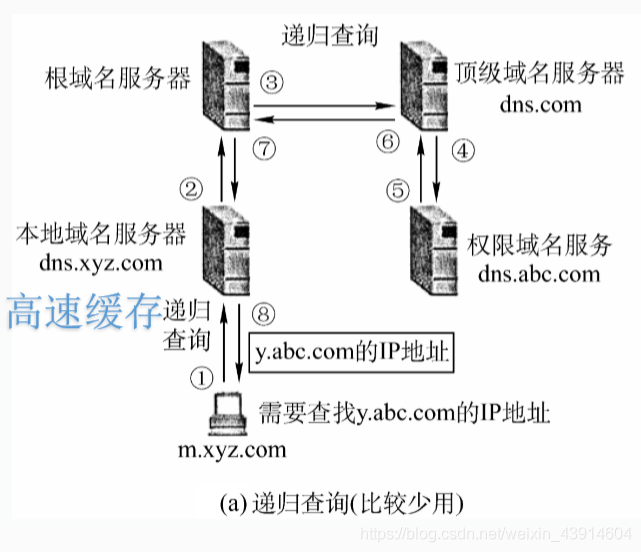
\includegraphics[width=.48\linewidth]{figures/digui.png}
    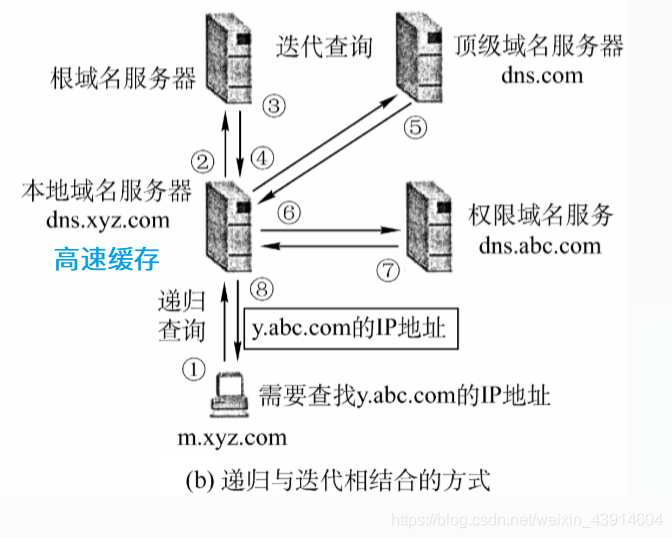
\includegraphics[width=.48\linewidth]{figures/diedai.png}
\end{figure}

\section{互联网的三种文档}

\begin{itemize}
    \item[1.] 静态文档
\end{itemize}

静态文档是指内容固定的文档，它是由万维网服务器创建，并存放在其中。

当客户利用浏览器访问万维网服务器里的该文档时，这个文档的副本被传送到客户，客户就可使用浏览程序显示这个文档。当然，服务器中的文档内容是可以修改的，但客户却不能修改它。

静态文档的最大优点是简单，文档可以由非程序设计人员来创建。它的缺点是不够灵活。因此，对于内容变化频繁的文档是不适合做成静态文档的。

\begin{itemize}
    \item[2.] 动态文档
\end{itemize}

所谓 “ 动态 ” ，并不是指网页的上动态效果，例如：视频、动图以及滚动字幕等。

所谓的动态网页，是指跟静态网页相对的一种网页编程技术。静态网页，随着html代码的生成，页面的内容和显示效果就基本上不会发生变化了——除非你修改页面代码。动态网页则不然，页面代码虽然没有变，但是显示的内容却是可以随着时间、环境或者数据库操作的结果而发生改变的。

动态文档是指文档的内容是在浏览器访问服务器时才得以创建。当浏览器的请求到达时，服务器就运行一个创建动态文档的应用程序。

动态文档的最大优点是具有告知当前最新信息的能力。

该应用程序对调览器发送来的数据进行处理，服务器把该程序或脚本的输出作为对浏览器请求该文档的响应。由于浏览器每次请求的响应都是动态生成的，因此每一个请求所得到的动态文档的内容也不一样。

\begin{itemize}
    \item[3.] 活动文档
\end{itemize}

活动文档是指能够提供了一种连续更新屏幕内容的技术，这种技术把创建文档的工作移到浏览器端进行。

当浏览器请求一个活动文档时，服务器就返回这个活动文档程序的副本或脚本，然后就在浏览器端运行，此时，活动文档程序可与用户直接交互，以便连续地更新屏幕的显示内容。

\begin{framed}
    静态文档和动态文档都是纯HTML文档，但是其产生的机制和静态万维网文档是有区别。
    
    活动文档是HTML的文档添加了其他的一些编程
\end{framed}


\section{计算机网络体系结构}

\subsection{计算机网络体系结构的形成}
计算机网络体系结构的形成计算机网络是个非常复杂的系统。为了说明这一点，可以设想一种最简单的情况：连接在网络上的两台计算机要互相传送文件。显然，在这两台计算机之间必须有一条传送数据的通路。但这还远远不够。至少还有以下几项工作需要去完成：
\begin{enumerate}
    \item 发起通信的计算机必须将数据通信的通路进行激活（activate）。所谓“激活”就是要发出一些信令，保证要传送的计算机数据能在这条通路上正确发送和接收。
    \item 要告诉网络如何识别接收数据的计算机。
    \item 发起通信的计算机必须查明对方计算机是否已开机，并且与网络连接正常。
    \item 发起通信的计算机中的应用程序必须弄清楚，在对方计算机中的文件管理程序是否已做好接收文件和存储文件的准备工作。
    \item 若计算机的文件格式不兼容，则至少其中一台计算机应完成格式转换功能。
    \item 对出现的各种差错和意外事故，如数据传送错误、重复或丢失，网络中某个结点交换机出现故障等，应当有可靠的措施保证对方计算机最终能够收到正确的文件。
\end{enumerate}

由此可见，相互通信的两个计算机系统必须高度协调工作才行，而这种“协调”是相当复杂的。为了设计这样复杂的计算机网络，早在最初的ARPANET设计时即提出了分层的方法。“分层”可将庞大而复杂的问题，转化为若干较小的局部问题，而这些较小的局部问题就比较易于研究和处理。

1974年，美国的IBM公司宣布了系统网络体系结构SNA（System Network Architecture）。这个著名的网络标准就是按照分层的方法制定的。现在用IBM大型机构建的专用网络仍在使用SNA。不久后，其他一些公司也相继推出自己公司的具有不同名称的体系结构。

不同的网络体系结构出现后，使用同一个公司生产的各种设备都能够很容易地互连成网。这种情况显然有利于一个公司垄断市场。但由于网络体系结构的不同，不同公司的设备很难互相连通。

然而，全球经济的发展使得不同网络体系结构的用户迫切要求能够互相交换信息。为了使不同体系结构的计算机网络都能互连，国际标准化组织ISO于1977年成立了专门机构研究该问题。他们提出了一个试图使各种计算机在世界范围内互连成网的标准框架，即著名的开放系统互连基本参考模型OSI/RM（Open Systems Interconnection Reference Model），简称为OSI，也就是所谓的七层协议的体系结构。

OSI试图达到一种理想境界，即全球计算机网络都遵循这个统一标准，因而全球的计算机将能够很方便地进行互连和交换数据。在20世纪80年代，许多大公司甚至一些国家的政府机构纷纷表示支持OSI。当时看来似乎在不久的将来全世界一定会按照OSI制定的标准来构造自己的计算机网络。然而到了20世纪90年代初期，虽然整套的OSI国际标准都已经制定出来了，但由于基于TCP/IP的互联网已抢先在全球相当大的范围成功地运行了，而与此同时却几乎找不到有什么厂家生产出符合OSI标准的商用产品。因此人们得出这样的结论：OSI只获得了一些理论研究的成果，但在市场化方面则事与愿违地失败了。现今规模最大的、覆盖全球的、基于TCP/IP的互联网并未使用OSI标准。

OSI失败的原因可归纳为：
\begin{enumerate}
    \item OSI的专家们缺乏实际经验，他们在完成OSI标准时缺乏商业驱动力；
    \item OSI的协议实现起来过分复杂，而且运行效率很低；
    \item OSI标准的制定周期太长，因而使得按OSI标准生产的设备无法及时进入市场；
    \item OSI的层次划分不太合理，有些功能在多个层次中重复出现。
\end{enumerate}

按照一般的概念，网络技术和设备只有符合有关的国际标准才能大范围地获得工程上的应用。但现在情况却反过来了。得到最广泛应用的不是法律上的国际标准OSI，而是非国际标准TCP/IP。这样，TCP/IP就常被称为是事实上的国际标准。从这种意义上说，能够占领市场的就是标准。在过去制定标准的组织中往往以专家、学者为主。但现在许多公司都纷纷加入各种标准化组织，使得技术标准具有浓厚的商业气息。一个新标准的出现，有时不一定反映其技术水平是最先进的，而是往往有着一定的市场背景。


\subsection{计算机网络的三种体系结构}

\begin{enumerate}
    \item OSI七层协议体系结构
    
    OSI是由国际标准化组织制定的标准，它概念清楚，理论完善，但是复杂又不实用。
    \item TCP/IP的四层协议
    
    TCP/IP体系结构得到了非常广泛的应用。它包含应用层、运输层、网际层和网络接口层（用网际层这个名字是强调这一层是为了解决不同网络的互连问题）。不过从实质上讲，TCP/IP只有最上面的三层，因为最下面的网络接口层并没有什么具体内容。
    \item 五层协议的体系结构
    
    学习计算机网络时我们一般采用折中的办法，也就是中和 OSI 和 TCP/IP 的优点，采用一种只有五层协议的体系结构，这样既简洁又能将概念阐述清楚。
\end{enumerate}

\subsection{各层的作用}

\begin{itemize}
    \item[1.] 应用层
\end{itemize}

应用层(application-layer)的任务是通过应用进程间的交互来完成特定网络应用。应用层协议定义的是应用进程（进程：主机中正在运行的程序）间的通信和交互的规则。对于不同的网络应用需要不同的应用层协议。在互联网中应用层协议很多，如域名系统DNS，支持万维网应用的 HTTP协议，支持电子邮件的 SMTP协议等等。我们把应用层交互的数据单元称为报文。

\begin{itemize}
    \item[2.] 运输层
\end{itemize}

运输层(transport layer)的主要任务就是负责向两台主机进程之间的通信提供通用的数据传输服务。应用进程利用该服务传送应用层报文。“通用的”是指并不针对某一个特定的网络应用，而是多种应用可以使用同一个运输层服务。由于一台主机可同时运行多个线程，因此运输层有复用和分用的功能。所谓复用就是指多个应用层进程可同时使用下面运输层的服务，分用和复用相反，是运输层把收到的信息分别交付上面应用层中的相应进程。

运输层主要使用以下两种协议

传输控制协议 TCP（Transmisson Control Protocol）--提供面向连接的，可靠的数据传输服务。

用户数据协议 UDP（User Datagram Protocol）--提供无连接的，尽最大努力的数据传输服务（不保证数据传输的可靠性）。

\begin{framed}
    \cred{TCP 的主要特点}

1. TCP 是面向连接的。（就好像打电话一样，通话前需要先拨号建立连接，通话结束后要挂机释放连接）；

2. 每一条 TCP 连接只能有两个端点，每一条TCP连接只能是点对点的（一对一）；

3. TCP 提供可靠交付的服务。通过TCP连接传送的数据，无差错、不丢失、不重复、并且按序到达；

4. TCP 提供全双工通信。TCP 允许通信双方的应用进程在任何时候都能发送数据。TCP 连接的两端都设有发送缓存和接收缓存，用来临时存放双方通信的数据；

5. 面向字节流。TCP 中的“流”（Stream）指的是流入进程或从进程流出的字节序列。“面向字节流”的含义是：虽然应用程序和 TCP 的交互是一次一个数据块（大小不等），但 TCP 把应用程序交下来的数据仅仅看成是一连串的无结构的字节流。
\end{framed}

\begin{itemize}
    \item[3.] 网络层
\end{itemize}

在计算机网络中进行通信的两个计算机之间可能会经过很多个数据链路，也可能还要经过很多通信子网。网络层的任务就是选择合适的网间路由和交换结点，确保数据及时传送。在发送数据时，网络层把运输层产生的报文段或用户数据报封装成分组和包进行传送。在 TCP/IP 体系结构中，由于网络层使用 IP 协议，因此分组也叫 IP 数据报 ，简称数据报。

网络层中的“网络”二字已经不是我们通常谈到的具体网络，而是指计算机网络体系结构模型中第三层的名称.

互联网是由大量的异构（heterogeneous）网络通过路由器（router）相互连接起来的。互联网使用的网络层协议是无连接的网际协议IP（Internet Protocol）和许多种路由选择协议，因此互联网的网络层也叫做网际层或IP层。网络层、网际层和IP层都是同义语。

\begin{itemize}
    \item[4.] 数据链路层
\end{itemize}

数据链路层(data link layer)通常简称为链路层。两台主机之间的数据传输，总是在一段一段的链路上传送的，这就需要使用专门的链路层的协议。 在两个相邻节点之间传送数据时，数据链路层将网络层交下来的 IP 数据报组装程帧，在两个相邻节点间的链路上传送帧。每一帧包括数据和必要的控制信息（如同步信息，地址信息，差错控制等）。

在接收数据时，控制信息使接收端能够知道一个帧从哪个比特开始和到哪个比特结束。这样，数据链路层在收到一个帧后，就可从中提出数据部分，上交给网络层。 控制信息还使接收端能够检测到所收到的帧中有误差错。如果发现差错，数据链路层就简单地丢弃这个出了差错的帧，以避免继续在网络中传送下去白白浪费网络资源。如果需要改正数据在链路层传输时出现差错（这就是说，数据链路层不仅要检错，而且还要纠错），那么就要采用可靠性传输协议来纠正出现的差错。这种方法会使链路层的协议复杂些。

\begin{itemize}
    \item[5.] 物理层
\end{itemize}

在物理层上所传送的数据单位是比特。 物理层(physical layer)的作用是实现相邻计算机节点之间比特流的透明传送，尽可能屏蔽掉具体传输介质和物理设备的差异。 使其上面的数据链路层不必考虑网络的具体传输介质是什么。“透明传送比特流”表示经实际电路传送后的比特流没有发生变化，对传送的比特流来说，这个电路好像是看不见的。

在互联网使用的各种协中最重要和最著名的就是 TCP/IP 两个协议。现在人们经常提到的TCP/IP并不一定单指TCP和IP这两个具体的协议，而往往表示互联网所使用的整个TCP/IP协议族。

\section{协议端口}

在网络技术中，端口（Port）有好几种意思。集线器、交换机、路由器的端口指的是连接其他网络设备的接口，如RJ-45端口、Serial端口等。我们 这里所指的端口不是指物理意义上的端口，而是特指TCP/IP协议中的端口，是逻辑意义上的端口。

如果把IP地址比作一间房子 ，端口就是出入这间房子的门。真正的房子只有几个门，但是一个IP地址的端口可以有65536（即：$2^{16}$）个之多！端口是通过端口号来标记的，端口号只有整数，范围是从0 到65535（$2^{16}-1$）。

在Internet上，各主机间通过TCP/IP协议发送和接收数据包，各个数据包根据其目的主机的ip地址来进行互联网络中的路由选择,把数据包顺利的传送到目的主机。大多数操作系统都支持多程序（进程）同时运行，那么目的主机应该把接收到的数据包传送给众多同时运行的进程中的哪一个呢？显然这个问题有待解决，端口机制便由此被引入进来。

本地操作系统会给那些有需求的进程分配协议端口（protocol port，即我们常说的端口），每个协议端口由一个正整数标识，如：80，139，445，等等。当目的主机接收到数据包后，将根据报文首部的目的端口号，把数据发送到相应端口，而与此端口相对应的那个进程将会领取数据并等待下一组数据的到来。

\begin{framed}
    \cred{TCP连接状态详解}

    LISTEN： 侦听来自远方的TCP端口的连接请求

SYN-SENT： 再发送连接请求后等待匹配的连接请求

SYN-RECEIVED：再收到和发送一个连接请求后等待对方对连接请求的确认

ESTABLISHED： 代表一个打开的连接

FIN-WAIT-1： 等待远程TCP连接中断请求，或先前的连接中断请求的确认

FIN-WAIT-2： 从远程TCP等待连接中断请求

CLOSE-WAIT： 等待从本地用户发来的连接中断请求

CLOSING： 等待远程TCP对连接中断的确认

LAST-ACK： 等待原来的发向远程TCP的连接中断请求的确认

TIME-WAIT： 等待足够的时间以确保远程TCP接收到连接中断请求的确认

CLOSED： 没有任何连接状态

\end{framed}

\begin{framed}
    \cred{查看端口命令 \quad netstat (选项)}

    -a或–all 列出所有端口(包含TCP和UDP)；

    -at 列出所有TCP端口

    -au 列出所有UDP端口

    -l 列出所有处于监听状态的端口

    -o 显示拥有的与每个连接关联的进程PID

\end{framed}

\section{TCP/IP多路复用}

所有网络通信的本质目标就是进程间通信。

除了寻址（Addressing），IP 协议还有一个非常重要的能力就是路由。
 寻址告诉我们去往下一个目的地该朝哪个方向走，路由则是根据下一个目的地选择路径。寻址更像在导航，路由更像在操作方向盘。

多路复用

 一台机器上的应用可以有很多。但是实际的出口设备，比如说网卡、网线通常只有一份。因此这里需要用到一个叫作多路复用（Multiplex）的技术。多路复用，就是多个信号，复用一个信道。

传输层多路复用

 多个请求复用一个 TCP 连接。

多个请求相当于并行的发送请求。即使其中某个请求发生故障，也不会阻塞其他请求。从这个角度看，多路复用实际上是一种 Non-Blocking（非阻塞）的技术。

如果其中一个数据段（TCP Segment）发生异常，只影响其中一个颜色的请求，其他请求仍然可以到达服务。

网络层多路复用

 两个应用之间的线路、设备，需要跨越的网络往往是固定的。在我们的互联网上，每时每刻都有大量的应用在互发消息。而这些应用要复用同样的基础建设——网线、路由器、网关、基站等。

应用层的多路复用，如多个请求使用同一个信道并行的传输，实际上是传输层提供的多路复用能力。传输层的多路复用，比如多个 TCP 连接复用一条线路，实际上是网络层在提供多路复用能力。

多路复用让多个信号（例如：请求/返回等）共用一个信道（例如：一个 TCP 连接）。它有两个明显的优势。
 提升吞吐量。多一个信号被紧密编排在一起（例如：TCP 多路复用节省了多次连接的数据），这样网络不容易空载。
 多个信号间隔离。信号间并行传输，并且隔离，不会互相影响。

\section{三次握手}

\cred{为什么要三次握手}

第一次握手：Client 什么都不能确认；Server 确认了对方发送正常。

第二次握手：Client 确认了：自己发送、接收正常，对方发送、接收正常；Server 确认了：自己接收正常，对方发送正常。

第三次握手：Client 确认了：自己发送、接收正常，对方发送、接收正常；Server 确认了：自己发送、接收正常，对方发送接收正常。

所以三次握手就能确认双发收发功能都正常，缺一不可。

\cred{SYN，ACK}

SYN (synchronous 建立联接 ) \qquad ACK(Acknowledgement 确认)

SYN 是 TCP/IP 建立连接时使用的握手信号。在客户机和服务器之间建立正常的 TCP 网络连接时，客户机首先发出一个 SYN 消息，服务器使用 SYN-ACK 应答表示接收到了这个消息，最后客户机再以 ACK消息响应。这样在客户机和服务器之间才能建立起可靠的TCP连接，数据才可以在客户机和服务器之间传递。

\section{四次挥手}

断开一个 TCP 连接则需要“四次挥手”：

客户端-发送一个 FIN，用来关闭客户端到服务器的数据传送

服务器-收到这个 FIN(finish 结束) ，它发回一个 ACK，确认序号为收到的序号加1 。和 SYN 一样，一个 FIN 将占用一个序号

服务器-关闭与客户端的连接，发送一个FIN给客户端

客户端-发回 ACK 报文确认，并将确认序号设置为收到序号加1

\cred{为什么要四次挥手}

任何一方都可以在数据传送结束后发出连接释放的通知，待对方确认后进入半关闭状态。当另一方也没有数据再发送的时候，则发出连接释放通知，对方确认后就完全关闭了TCP连接。

举个例子：A 和 B 打电话，通话即将结束后，A 说“我没啥要说的了”，B回答“我知道了”，但是 B 可能还会有要说的话，A 不能要求 B 跟着自己的节奏结束通话，于是 B 可能又巴拉巴拉说了一通，最后 B 说“我说完了”，A 回答“知道了”，这样通话才算结束。

\section{TCP 可靠通信的具体实现}

TCP发送的报文段是交给IP层传送的，但IP层只能提供尽最大努力交付的服务，也就是说，TCP下面的网络所提供的是不可靠的传输。因此，TCP采用了一些适当的措施来提供可靠的传输，使得两个传输层直接的通信变得可靠。

TCP协议通过使用连续ARQ协议和滑动窗口协议，来保证数据传输的正确性，从而提供可靠的传输。

{\bfseries \cgreen{ARQ协议}}

ARQ协议，即自动重传请求（Automatic Repeat-reQuest），是OSI模型中数据链路层和传输层的错误纠正协议之一。它通过使用确认和超时这两个机制，在不可靠服务的基础上实现可靠的信息传输。如果发送方在发送后一段时间之内没有收到确认帧，它通常会重新发送。ARQ包括停止等待ARQ协议和连续ARQ协议。

{\bfseries \cgreen{停止等待ARQ协议}}

要想弄明白为什么TCP要使用连续ARQ协议，首先需要弄清楚停止等待ARQ协议的原理。

A发送分组M1，发送完就暂停发送，等待B的确认。B收到M1就向A发送确认。A在收到了对M1的确认后，就再发送下一个分组M2。依次下去发送剩余的数据...

如果A发送的过程中出现差错，B在接收M1时检测出了差错，就丢弃M1，其他什么都不做（也不会通知A收到有差错的分组）。又或者A传送的过程中分组丢失了，以上这两种情况下，B不会发送任何信息。 

既然说它是可靠传输协议，那自然有它可靠的方法：如果发生以上的情况，A只要超过了一段时间仍然没有收到确认，就认为刚才发送的分组丢失了，所以它会重传刚刚的发送过的分组，也就是所谓的超时重传。 

\begin{figure}[ht]
    \centering
    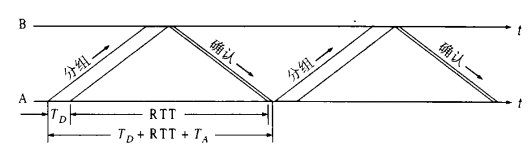
\includegraphics[]{figures/ARQ1.png}
\end{figure}

停止等待ARQ协议的优点是简单，但也有很严重的缺点，就是信道利用率太低。

{\bfseries \cgreen{连续ARQ协议}}

由于停止等待ARQ协议信道利用率太低，所以需要使用连续ARQ协议来进行改善。这个协议会连续发送一组数据包，然后再等待这些数据包的ACK。发送方采用流水线传输。流水线传输就是发送方可以连续发送多个分组，不必每发完一个分组就停下来等待对方确认。

\begin{figure}[ht]
    \centering
    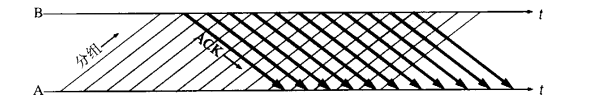
\includegraphics[]{figures/ARQ2.png}
\end{figure}

连续ARQ协议通常是结合滑动窗口协议来使用的，发送方需要维持一个发送窗口，位于发送窗口内的5个分组都可以连续发送出去，而不需要等待对方的确认，这样就提高了信道利用率。 

连续ARQ协议规定，发送方每收到一个确认，就把发送窗口向前滑动一个分组的位置。

接收方一般都是采用累积确认的方式。也就是说接收方不必对收到的分组逐个发送确认。而是在收到几个分组后，对按序到达的最后一个分组发送确认。如果收到了这个分组确认信息，则表示到这个分组为止的所有分组都已经正确接收到了。 

\begin{figure}[ht]
    \centering
    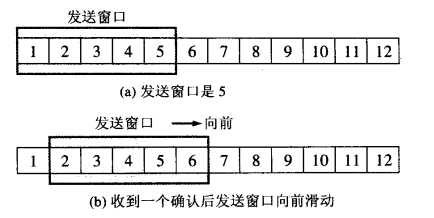
\includegraphics[]{figures/ARQ3.png}
\end{figure}

\section{TCP报文段首部格式}

\begin{figure}[ht]
    \centering
    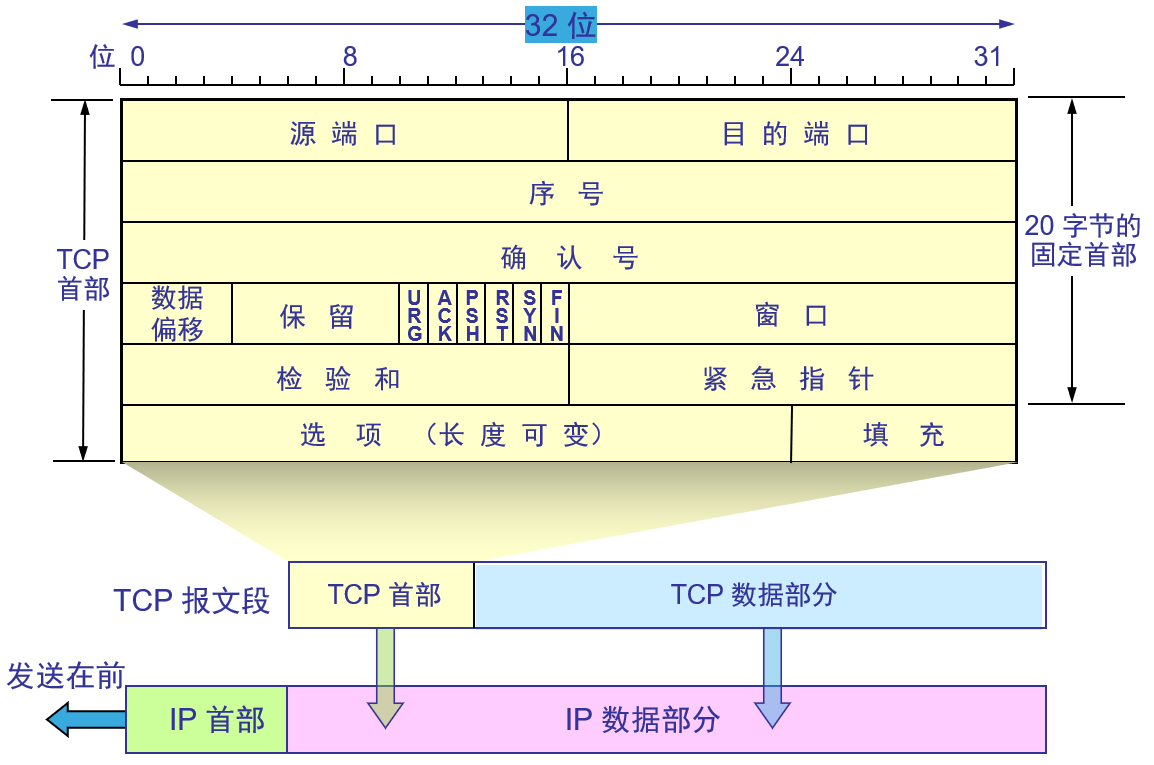
\includegraphics[width=.9\linewidth]{figures/TCP.png}
\end{figure}

源端口和目的端口：各占2个字节，建立端口用

序号：4个字节，用来给TCP传输中的字节流编号，传输的每个字节都要按顺序编号，循环使用。范围是$[0, 2^{32}-1]$。报文段的序号由要传送的字节路中的第一个字节的序号决定，例如序号字段值为301，携带100字节，那么下一个报文段数据序号从401开始，序号字段值为401

确认号：4字节长度，期望收到对方下一个报文段的第一个数据字节的序号；例如确认号是701，那么说明已经接收到了序号到700为止的数据

检验和：占2字节，检验范围包括首部和数据2部分。

紧急指针：占2字节，URG=1时才有用。用来指出本报文段中的紧急数据的字节数

选项：长度可变，最长40字节。没有这个的时候TCP首部长度为20字节

\begin{framed}
    {\bfseries \cgreen{TCP的六个控制位}}

    紧急位URG：URG的特点就是让数据插队，URG=1的就会在缓存中被提前到第一个传输

    确认位ACK

    推送位PSH：就是接收端的URG，将PSH=1的数据尽快接收

    复位RST：RST=1时，表明TCP连接中出现严重差错，必须释放连接，然后再重新建立传输链接。

    同步位SYN

    终止位FIN
\end{framed}

\section{UDP的首部格式}

\begin{figure}[ht]
    \centering
    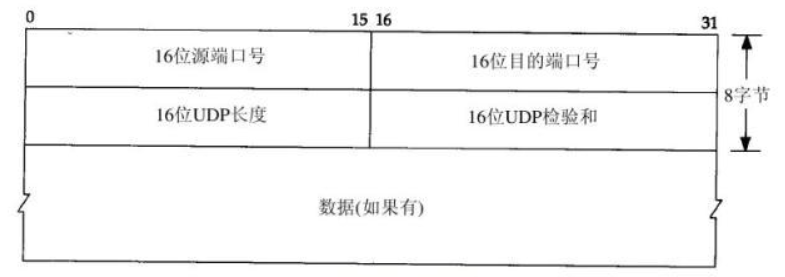
\includegraphics[width=.9\linewidth]{figures/UDP.png}
\end{figure}

源端口：端口号0-65535，1-1024保留端口号，为标准的服务端口

目的端口：无须多解释

UDP长度：header + data 总长度

UDP校验和：伪头部，头部，data 三部分校验和。

数据：上层应用层的数据。

伪头部：UDP校验和中的伪头部，并非UDP报文中的有效数据，是提取了IP数据报中的源IP，目的IP信息并加上协议等字段构造的数据。伪头部在实际网络传输中，仅用作校验和计算使用，并不发送！因此称为伪头部。事实上在TCP校验和计算中也用到了伪头部，与UDP一致。


\section{ARP 地址解析协议}

ARP作用：IP地址解析为MAC地址

为什么需要MAC地址才能通信？

通过之前的OSI七层模型可以知道，数据在数据链路层传输的时候会加一个帧的头部，里面包含MAC地址，解封的过程也需要MAC地址。

\begin{figure}[ht]
    \centering
    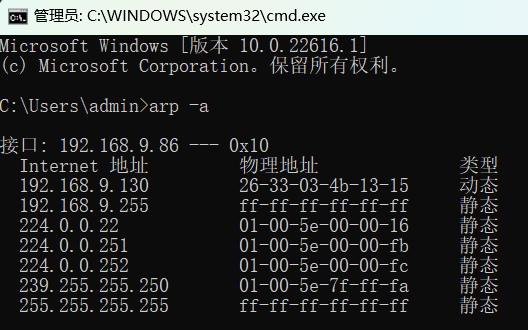
\includegraphics[]{figures/ARP.png}
    \caption{ARP缓存表\ 指令 arp -a}
\end{figure}

ARP缓存表是主机最近运行时获得关于其他主机的IP地址到MAC地址的映射，当需要发送数据的时候，主机就会根据数据报中的目标IP地址信息，然后在ARP缓存表中进行查找对应的MAC地址，最后通过网卡将数据发送出去。

如果没有查到，就向本地网段发起一个ARP请求的广播包，查询此目的主机对应的MAC地址。此ARP请求数据包里包括源主机的IP地址、硬件地址、以及目的主机的IP地址。网络中所有的主机收到这个ARP请求后，会检查数据包中的目的IP是否和自己的IP地址一致。如果不相同就忽略此数据包；如果相同，该主机首先将发送端的MAC地址和IP地址添加到自己的ARP列表中，如果ARP表中已经存在该IP的信息，则将其覆盖，然后给源主机发送一个 ARP响应数据包，告诉对方自己是它需要查找的MAC地址；源主机收到这个ARP响应数据包后，将得到的目的主机的IP地址和MAC地址添加到自己的ARP列表中，并利用此信息开始数据的传输。如果源主机一直没有收到ARP响应数据包，表示ARP查询失败。

\begin{figure}[ht]
    \centering
    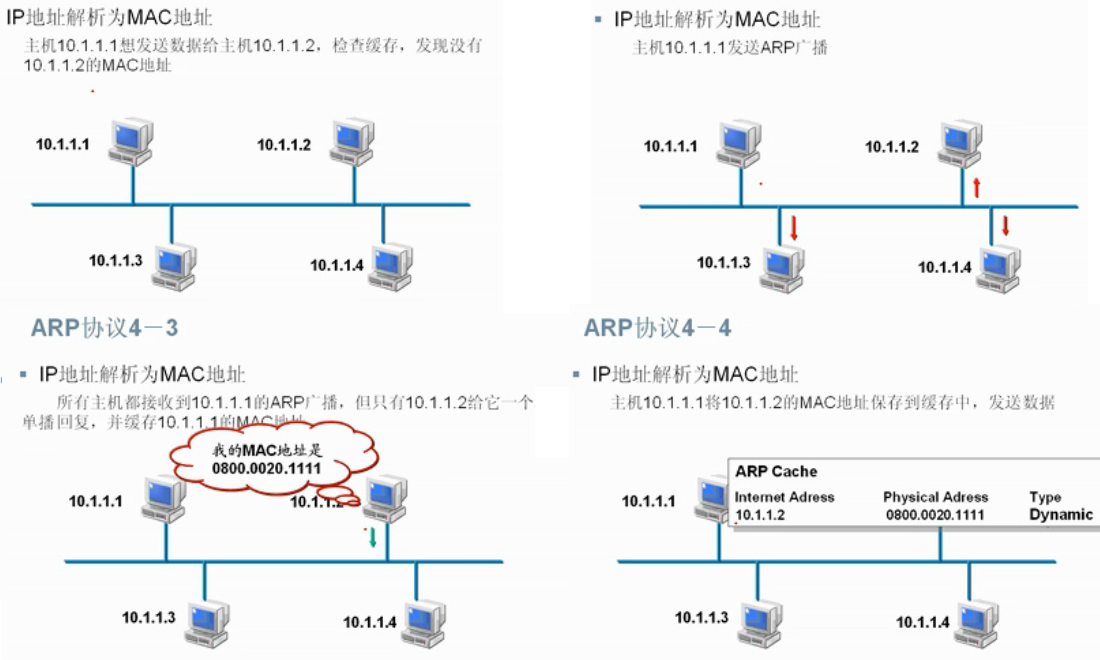
\includegraphics[width=\linewidth]{figures/ARP2.png}
\end{figure}

\section{链路层}

物理层解决了信号传输的环境问题，简单理解就是传输了各种信号，但是双方都不能理解对方发来的信号的意思，链路层就是规定一种协议(信号是谁发的，给谁的，数据部分哪里开始哪里结束的)，使得通信双方能够正常交流。

平常我们说话都是一句一句的，这在链路层中以帧为单位进行传送，另外在通信过程中会产生(距离远，有人干扰信号)一些问题，所以引入了透明传输与差错检测两种机制。

MAC尾部的FCS就是差错检测的手段，发往本站的MAC帧被收下之后，校验范围从目的地址段到数据段的末尾，算法采用32位循环冗余码（CRC），不但需要检验MAC帧的数据部分，还要检验目的地址，源地址和类型字段，但不校验前导码。

世界上每块网卡都有一个唯一的地址，即MAC地址，因为以太网逻辑上采用总线型拓扑结构，即以太网中所有计算机共享一条总线，信息以广播方式发送，因此网卡从网络上每收到一个MAC帧，首先要用硬件检查MAC帧中的MAC地址，如果是发往本站的帧才会收下，否则丢弃。


\section{虚拟专用网 VPN}

虚拟专用网络(VPN)是一门新型的网络技术，它为我们提供了一种通过公用网络(如最大的公用因特网)安全地对企业内部专用网络进行远程访问的连接方式。

我们知道一个网络连接通常由三个部分组成：客户机、传输介质和服务器。VPN网络同样也需要这三部分，不同的是VPN连接不是采用物理的传输介质，而是使用一种称之为“隧道”的东西来作为传输介质的，这个隧道是建立在公共网络或专用网络基础之上的，如因特网或专用Intranet等。

要实现VPN连接，企业内部网络中必须配置有一台VPN服务器，VPN服务器一方面连接企业内部专用网络(LAN)，另一方面要连接到因特网或其它专用网络，这就要VPN服务器必须拥有一个公用的IP地址，也就是说企业必须先拥有一个合法的Internet或专用网域名。

整个VPN通信过程可以简化为以下4个通用步骤：

(1)客户机向VPN服务器发出请求；

(2) VPN服务器响应请求并向客户机发出身份质询，客户机将加密的用户身份验证响应信息发送到VPN服务器；

(3) VPN服务器根据用户数据库检查该响应，如果账户有效，VPN服务器将检查该用户是否具有远程访问权限；如果该用户拥有远程访问的权限，VPN服务器接受此连接；

(4)最后VPN服务器将在身份验证过程中产生的客户机和服务器公有密钥将用来对数据进行加密，然后通过VPN隧道技术进行封装、加密、传输到目的内部网络。